%# -*- coding: utf-8 -*-
%\documentclass [b5paper,12pt,openany]{book}
\documentclass [a4paper,12pt,openany]{book}

\usepackage[italian]{babel}
\usepackage[utf8]{inputenc}
\usepackage[T1]{fontenc}
\usepackage{lmodern}
\usepackage{graphicx}
\usepackage{listings}

\usepackage{times} %impostazione font
\renewcommand{\familydefault}{\sfdefault} %attivazione nuovo font

\begin{document}
\pagestyle{empty}
\setlength{\parindent}{0pt} %elimina indentazione prima linea paragrafi
\setlength{\parskip}{6pt} %distanza verticale tra due paragrafi
\noindent

\begin{minipage}[c][\textheight][c]{\textwidth}\centering
\textsc{\Large Nadia}
\vfill
\textbf{\Huge ESEMPIO}
\vfill
\Large\oldstylenums{2010}
\end{minipage}

\newpage

\begin{minipage}[c][\textheight][c]{\textwidth}
\copyright2010 Nadia
\vspace{20mm}
Stampato in proprio\\
Soggetto alla licenza Creative Commons\\
Finito di stampare il 4 febbraio 2010
\end{minipage}
\newpage

\pagestyle{plain}
\tableofcontents

\listoffigures

\chapter{Un piccolo esempio}
\section{Un paragrafo o {\em section}\ldots}
\subsection{\ldots e un sottoparagrafo o {\em subsection}}
\section{Secondo paragrafo}
Con un pò di testo.
\subsection{Come vedete\ldots}
\subsubsection{Un sotto"sotto"paragrafo o {\em subsubsection}}
I sotto"sotto"paragrafi non compaiono nell'indice!

\chapter{Il mio primo capitolo}
Essere o non essere questo è il problema
\section{La mia prima sezione}

Io non so se funzionasse, ma proviamo ugualmente.

Proverò anche a lasciare una linea vuota. 

Ovviamente è possibile scegliere il tipo di formattazione che si desidera avere per il codice sorgente nel file .tex, specificando i colori delle parole chiave e lo stile del testo, per esempio, ma per questo rimando alla guida per l'utilizzo del pacchetto listings. Niente di più semplice questa volta e se l'avessi saputo anche l'anno scorso avrei di certo risparmiato un sacco di tempo! Purtroppo per qualche motivo non sono arrivata ad utilizzare questa soluzione, ma l'importante è aver risolto comunque, perché adesso mi posso rifare. :D Come sempre dire che LaTeX è difficile da usare significa non sapere di cosa si sta parlando!

\chapter{Il mio secondo capitolo}
Ma che bello questo sistema
\section{La seconda sezione}

Di seguito inserisco una immagine
	\begin{figure}[htbp]
	\centering
%	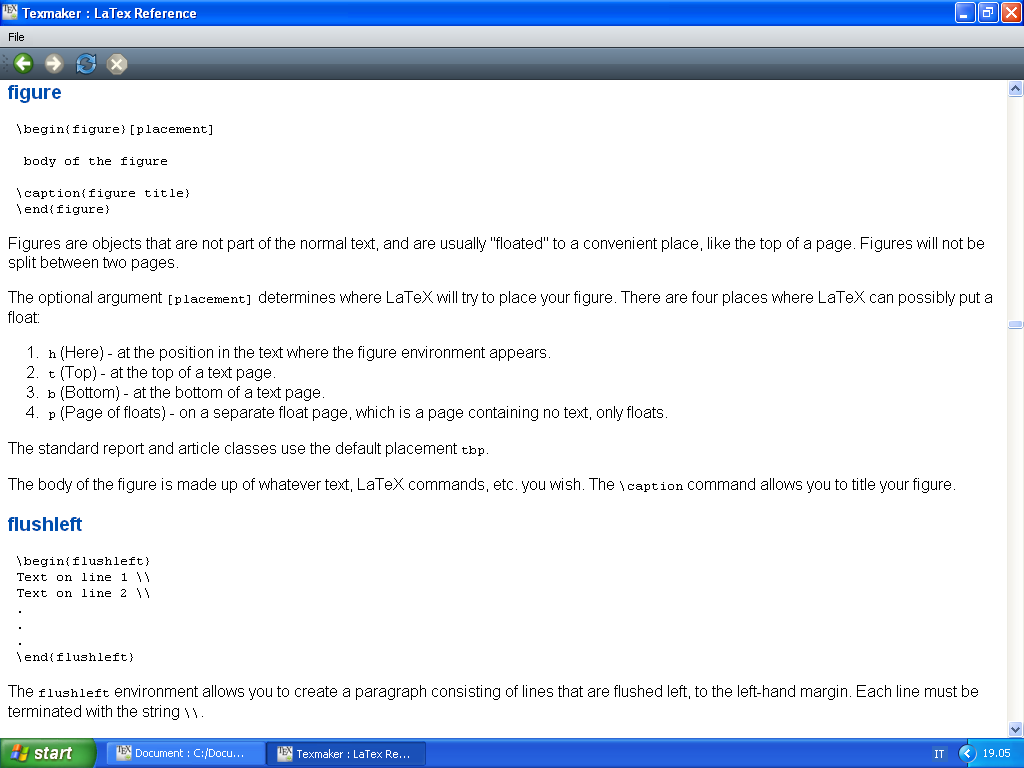
\includegraphics[width=\textwidth]{test.png}
	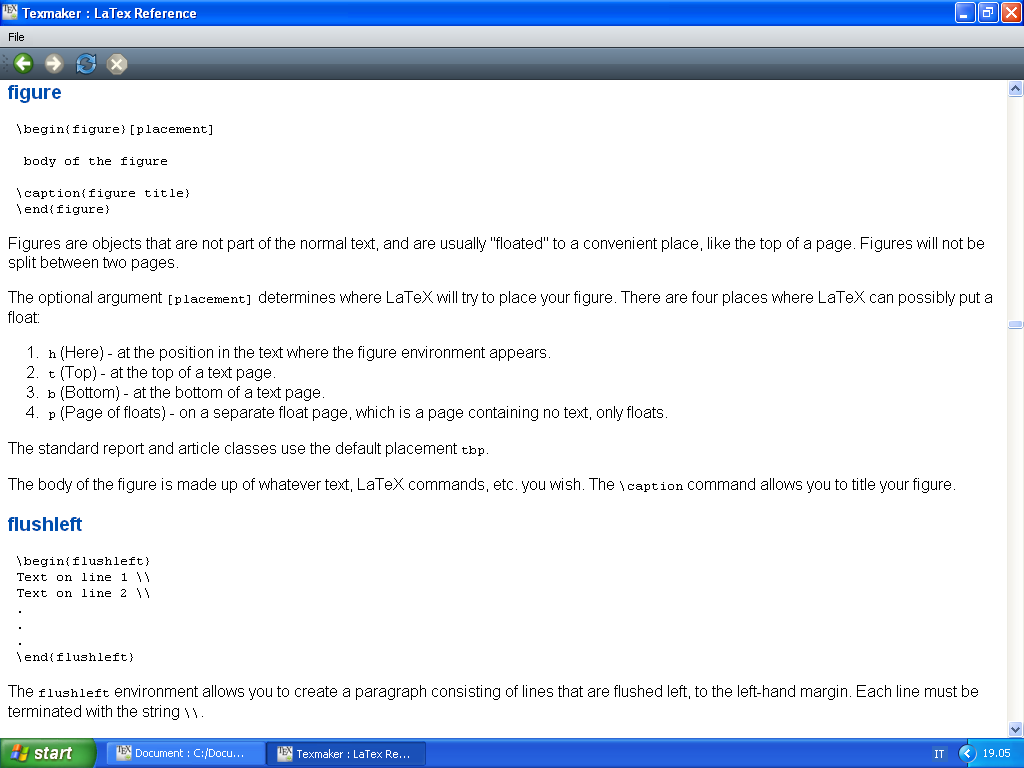
\includegraphics[width=10cm]{test.png}
	\caption{La mia figura test}\label{figura1}
	\end{figure}
\clearpage

Essere o non essere questo è il problema 2
Che bella la seconda sezione
Ovviamente è possibile scegliere il tipo di formattazione che si desidera avere per il codice sorgente nel file .tex, specificando i colori delle parole chiave e lo stile del testo, per esempio, ma per questo rimando alla guida per l'utilizzo del pacchetto listings. Niente di più semplice questa volta e se l'avessi saputo anche l'anno scorso avrei di certo risparmiato un sacco di tempo! Purtroppo per qualche motivo non sono arrivata ad utilizzare questa soluzione, ma l'importante è aver risolto comunque, perché adesso mi posso rifare. :D Come sempre dire che LaTeX è difficile da usare significa non sapere di cosa si sta parlando!

Ovviamente è possibile scegliere il tipo di formattazione che si desidera avere per il codice sorgente nel file .tex, specificando i colori delle parole chiave e lo stile del testo, per esempio, ma per questo rimando alla guida per l'utilizzo del pacchetto listings. Niente di più semplice questa volta e se l'avessi saputo anche l'anno scorso avrei di certo risparmiato un sacco di tempo! Purtroppo per qualche motivo non sono arrivata ad utilizzare questa soluzione, ma l'importante è aver risolto comunque, perché adesso mi posso rifare. :D Come sempre dire che LaTeX è difficile da usare significa non sapere di cosa si sta parlando!

%\lstloadlanguages{NOME_LINGUAGGIO}
\lstinputlisting{test.cpp}

\chapter{Il mio terzo capitolo}
Ma che bello questo sistema che mi permette di separare facilmente i capitoli
\section{La terza sezione}
Ecco il contenuto del nuovo file tex

\end{document}